% Este arquivo .tex será incluído no arquivo .tex principal. Não é preciso
% declarar nenhum cabeçalho

\section{Lugares para morar}

O custo de moradia em Barão Geraldo depende principalmente de três fatores:
proximidade da Unicamp, tamanho do imóvel e qualidade da casa (acabamento,
número de banheiros, presença de piscina etc.) Quanto à distância, os entornos da
\textbf{Avenida 1} (Avenida Doutor Romeu Tortima) e da \textbf{Avenida 2}
(Avenida Professor Atílio Martini) costumam ser mais caros de se morar, por serem
próximos da Unicamp. A região que vai do centro de Barão Geraldo até a Moradia
Estudantil, um pouco mais distante da universidade (cerca de 10 minutos de
bicicleta), é em geral mais barata e concentra muito mais serviços, como
supermercados, restaurantes e bancos.

Uma boa dica para se informar a respeito de lugares para morar (repúblicas,
quitinetes, pensionatos) é o site \textbf{Morar Unicamp}
(\url{morarunicamp.com.br}), criado por alunos. Lá você encontra informações
como endereço, preço, contato e detalhamento do lugar.

\subsection{Moradia Estudantil}

A \textbf{Moradia} é um exemplo de conquista de todos os estudantes. O processo
de reivindicação de uma moradia estudantil para a Unicamp começou com o
movimento Taba. Durante dois anos, alunos ficaram acampados no CB (Ciclo
Básico) até que as obras começassem. Hoje em dia, graças à Moradia, várias
pessoas que não teriam condições de se manter em Campinas pagando aluguel podem
estudar na Unicamp.

\begin{figure}[h!]
    \centering
    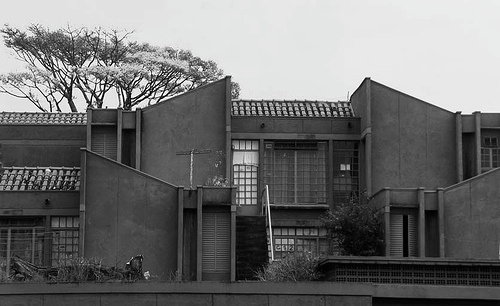
\includegraphics[scale=0.55,keepaspectratio=true]{img/imgs/5-moradia/-029.jpg}
\end{figure}

A Moradia existe desde 1989. De lá para cá, o número de vagas em cursos da
Unicamp aumentou muito e as vagas da Moradia tornaram-se insuficientes para
acomodar todos que precisam. A reivindicação de mais vagas para a Moradia é uma
das principais bandeiras do DCE e um desejo de muitos estudantes.

Cada casa da Moradia, normalmente dividida por quatro pessoas, constitui-se de
um quarto, uma cozinha, um banheiro e uma sala. Há ainda o Ônibus da Moradia, um
circular da Unicamp que transporta pessoas durante o dia todo da Moradia até a
Unicamp e vice-versa.

A Moradia está localizada na Avenida Santa Isabel, 1125, a cerca de 3 km do
campus.

Para saber mais sobre a Moradia e o processo seletivo, entre no site
\url{www.pme.unicamp.br}.

\subsection{Repúblicas}

A melhor escolha, se você tiver condições de pagar por uma moradia.

\begin{figure}[h!]
    \vspace{-10pt}
    \centering
    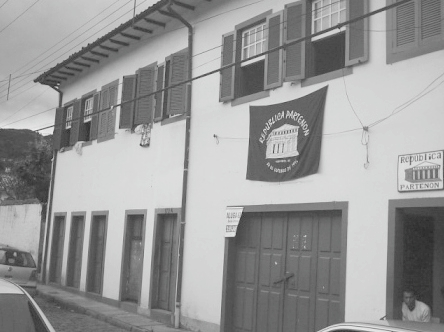
\includegraphics[scale=0.58,keepaspectratio=true]{img/imgs/5-moradia/-034.jpg}
    \vspace{-10pt}
\end{figure}

Você pode levar quem quiser para sua casa, chegar no horário que bem entender,
além do que você conhecerá muita gente nova. Se possível, more em uma república
de cursos mistos, pois assim você terá contatos diversos.

O custo de uma vaga em república é muito variável, a depender do conforto que
você espera e da localização. Gira em torno de R\$ 475 para dividir quarto com
outras pessoas e R\$ 650 para um quarto individual. Esses valores já são a soma
do aluguel com despesas adicionais (água, luz, limpeza etc.)

Escolha bem as pessoas com quem você vai morar para não ter problemas com
diferentes estilos de vida. Tem gente que gosta de lavar louça a cada 5 minutos
e tem gente que usa o chão como lata de lixo tranquilamente. Veja com quem você
se dá melhor.

\subsection{Quitinetes}

Cuidado! A especulação imobiliária em Barão Geraldo chega a ser imbecil. As
quitinetes mobiliadas são normalmente compostas de um banheiro e um cômodo que é
quarto, sala, cozinha e área de serviço. Os valores de aluguel são da ordem de
R\$ 1000 ou mais. Sim, mil reais por um microespaço. Só porque é perto da
Unicamp. Fique de olho e tome cuidado com os contratos.

\begin{figure}[h!]
    \centering
    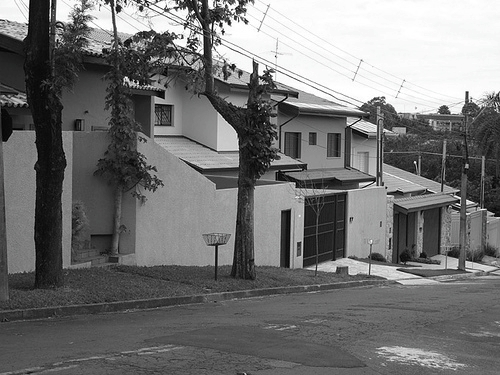
\includegraphics[scale=0.55,keepaspectratio=true]{img/imgs/5-moradia/-033.jpg}
\end{figure}

As melhores relações custo-benefício de quitinetes são as daquelas próximas ao
centro de Barão Geraldo ou no espaço entre as avenidas. E lembre-se de que não é
só de Unicamp que se vive. Não adianta pagar mais caro para estar do lado da
universidade, se você fica muito longe dos supermercados, farmácias etc.

\subsection{Pensionatos}

Pensionatos são como repúblicas, só que com regras. Muitas regras. Dependendo
do pensionato que você conseguir, pode tornar-se uma grande roubada. Alguns não
deixam você levar pessoas para casa, reclamam se você chegar tarde e não liberam
festas; outras, não, então procure bem.

O preço fica por volta de R\$ 625 para dividir quarto e R\$ 850 para quarto
individual. Pode ser uma opção muito cômoda se você procura um conjunto de casa,
comida e roupa lavada.

É muito importante que você saiba que contratos de um ano (ou qualquer período)
em pensionatos são ilegais e você não precisa cumpri-los.

\subsection{Segurança}

Por ter muitas casas de famílias abastadas e de estudantes (em geral desatentos),
Barão Geraldo é grande alvo de assaltos a residências e, além disso, o distrito
peca pela falta de segurança.

Não é raro ouvir que alguém foi assaltado enquanto voltava para casa à noite
sozinho ou que teve a casa saqueada durante um feriado prolongado. Mais chocantes
ainda são os casos de estupro de moças que ocasionalmente são divulgados em
grupos de e-mail e redes sociais. Cuidado! É importante zelar pela sua
integridade e pela de seus pertences -- assim como seus pais fazem em sua casa,
não importa onde eles morem.

\begin{figure}[h!]
    \centering
    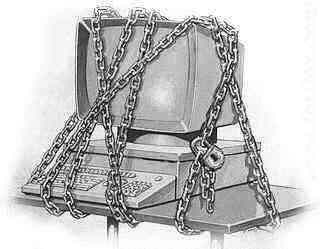
\includegraphics[scale=0.55,keepaspectratio=true]{img/imgs/5-moradia/seguranca.jpg}
\end{figure}

Evite andar sozinho à noite, especialmente nos fins de semana. Se o seu
pensionato ou a sua república paga o segurança da rua, o que é altamente
recomendável, use \emph{sempre} de seus serviços, seja ligando para pedir
escolta ao chegar em casa ou para avisar caso ouça algum barulho suspeito.

Ao voltar para sua cidade em feriados prolongados, deixando a casa vazia, não se
esqueça de trancar todas as portas e janelas de casa, verificar se não há nada
no quintal que possa ser levado facilmente (colocar as bicicletas e aparelhos de
som na sala é uma boa ideia) e trancar os objetos de valor (computadores,
televisões) dentro dos quartos.

\subsection{Imobiliárias}

\begin{itemize}
\item   \textbf{Imobiliária Barão Housing}
        \\Telefone: (19) 3289-4113
        \\Endereço: Rua Tranquilo Prosperi, 383
        \\E-mail: \email{atendimento@baraohousing.com.br}
        \\Site: \url{baraohousing.com.br}

\item   \textbf{Imobiliária Lanza}
		\\Endereço: Rua Benedito Alves Aranha, 104
		\\Telefone: (19) 3289-1717 / (19) 3307-7155
		\\E-mail: \email{lanza@lanzaimoveis.com.br}
		\\Site: \url{lanzaimoveis.com.br}

\item   \textbf{Imobiliária Professor Sebastião}
		\\Endereço: Av. Dr. Romeu Tortima, 344
		\\Telefone: (19) 3289-2317
		\\E-mail: \email{ipsimoveis@ipsimoveis.com.br}
		\\Site: \url{ipsimoveis.com.br}

\item   \textbf{Amaral Imóveis}
		\\Endereço: Av. Dr. Luiz de Tella, 864
		\\Telefone: (19) 3287-0655 / (19) 4141-1010
		\\E-mail: \email{amaral@amaralimoveis.net}
		\\Site: \url{amaralimoveis.net}

\item   \textbf{Zaine Conquista Imóveis}
		\\Endereço: Av. Santa Isabel, 84
		\\Telefone: (19) 3289-4050 / (19) 3289-2761
		\\E-mail: \email{zaine@correionet.com.br}
		\\Site: \url{zaineconquista.com.br}

\item   \textbf{Ismê Assessoria Imobiliária}
		\\Endereço: Rua Christina G. Miguel, 250
		\\Telefone: (19) 3289-4325
		\\E-mail: \email{isme@isme.com.br}
		\\Site: \url{isme.com.br}

\item   \textbf{Rute Svartman Imóveis}
		\\Endereço: Rua Engenheiro Edward de Vita Godoy, 850
		\\Telefone: (19) 3368-0881
		\\E-mail: \email{imoveis@rutesvartman.com.br}
		\\Site: \url{rutesvartman.com.br}

\item   \textbf{Imobiliária Ávila \& Ferraris}
		\\Endereço: Av. Dr. Romeu Tortima, 714
		\\Telefone: (19) 3289-3522
		\\E-mail: \email{dcaavila@terra.com.br}
		\\Site: \url{avilaeferrarisimoveis.com.br}

\item   \textbf{Imobiliária Cidade Universitária}
		\\Endereço: Av. Dr. Romeu Tortima, 624
		\\Telefone: (19) 3289-3322
		\\E-mail: \email{contato@cidadeuniversitariaimoveis.com.br}
		\\Site: \url{cidadeuniversitariaimoveis.com.br}

\item   \textbf{Denilson Imóveis}
		\\Endereço: Av. Dr. Luís de Tella, 55
		\\Telefone: (19) 3289-1444
		\\E-mail: \email{contato@denilsonimoveis.com.br}
		\\Site: \url{denilsonimoveis.com.br}

\item   \textbf{Mega Barão Imóveis}
		\\Endereço: Rua Francisca Resende Merciai, 103 B
		\\Telefone: (19) 3289-7101 / (19) 3386-4141
		\\E-mail: \email{megabarao@megabaraoimoveis.com.br}
		\\Site: \url{megabaraoimoveis.com.br}

\item   \textbf{Libano Imóveis}
		\\Endereço: Rua Francisca Resende Merciai, 90
		\\Telefone: (19) 3789-9999
		\\E-mail: \email{contato@libanoimoveis.com.br}
		\\Site: \url{libanoimoveis.com.br}

\item   \textbf{Marco Imóveis}
		\\Endereço: Rua José Pugliesi Filho, 420
		\\Telefone: (19) 3287-8083
		\\Site: \url{marcoimovel.com.br}

\item   \textbf{Lokal Imóveis}
		\\Endereço: Rua José Próspero Jacobucci, 290
		\\Telefone: (19) 3256-4616

\item   \textbf{Carpe Diem Imóveis}
		\\Endereço: Av. Dr. Romeu Tortima, 184
		\\Telefone: (19) 3579-5655 / (19) 3304-9323
		\\Site: \url{carpediemimoveis.com.br}

\item   \textbf{Cássio Carvalho Imóveis}
		\\Endereço: Av. Santa Isabel, 750
		\\Telefone: (19) 3288-0143
		\\E-mail: \email{cassio@cassioimoveis.com.br}
		\\Site: \url{cassioimoveis.com.br}

\item   \textbf{Delphos Empreendimentos Imobiliários}
        \\Endereço: Av. Albino J. B. de Oliveira, 830
        \\Telefone: (19) 3289-5353

\item   \textbf{Roma Imóveis}
        \\Endereço: Rua Agostinho Pattaro, 222
        \\Telefone: (19) 3287-9118

\item   \textbf{Valter Imóveis}
        \\Endereço: Rua Maria Ferreira Antunes, 22
        \\Telefone: (19) 3289-6088

\item   \textbf{Imobiliária Marco Antônio}
        \\Endereço: Av. Dr. Romeu Tortima, 1522
        \\Telefone: (19) 3287-6663
\end{itemize}
